\documentclass[a4paper,ngerman,12pt]{scrartcl}

\usepackage[utf8]{inputenc}
%\usepackage[ansinew]{inputenc}

\usepackage[ngerman]{babel}

\usepackage{amsmath,amsthm,amssymb,stmaryrd,color,graphicx}
\usepackage{setspace}
\usepackage{bussproofs}
\usepackage{array}
\usepackage{comment}
\usepackage{wrapfig}

\usepackage{enumitem}

\usepackage{units}

\usepackage[protrusion=true,expansion=true]{microtype}

\usepackage{lmodern}

\usepackage{hyperref}
\usepackage{cleveref}

\newcommand{\RR}{\mathbb{R}}
\newcommand{\CC}{\mathbb{C}}
\newcommand{\ZZ}{\mathbb{Z}}
\newcommand{\NN}{\mathbb{N}}
\newcommand{\QQ}{\mathbb{Q}}

\setlength\parskip{\medskipamount}
\setlength\parindent{0pt}

\theoremstyle{definition}
\newtheorem{defn}{Definition}[]
\newtheorem{axiom}[defn]{Axiom}
\newtheorem{bsp}[defn]{Beispiel}

\theoremstyle{plain}
\newtheorem{prop}[defn]{Proposition}
\newtheorem{motto}[defn]{Motto}
\newtheorem{wunder}[defn]{Wunder}
\newtheorem{ueberlegung}[defn]{Überlegung}
\newtheorem{lemma}[defn]{Lemma}
\newtheorem{kor}[defn]{Korollar}
\newtheorem{hilfsaussage}[defn]{Hilfsaussage}
\newtheorem{satz}[defn]{Satz}
\newtheorem{frage}[defn]{Frage}

\theoremstyle{remark}
\newtheorem{bem}[defn]{Bemerkung}
\newtheorem{aufg}[defn]{Aufgabe}

\newtheorem*{antwort}{Antwort}

\newlength{\aufgabenskip}
\setlength{\aufgabenskip}{1.4em}
\newcounter{aufgabennummer}
\newenvironment{aufgabe}[1]{
	\addtocounter{aufgabennummer}{1}
	\textbf{Aufgabe \theaufgabennummer.} \emph{#1} \par
}{\vspace{\aufgabenskip}}

\clubpenalty=10000
\widowpenalty=10000
\displaywidowpenalty=10000

\setlength\unitlength{1cm}

\usepackage{tikz}

\RequirePackage{geometry}
\geometry{textwidth=16.0cm,textheight=24.5cm,footskip=1.5cm}

\begin{document}
	
\begin{picture}(0,0)
\put(0,-0.5){%
	\includegraphics[scale=0.1]{logo-ifm}
}
\put(14.0,-3.5){%
	\includegraphics[scale=0.17]{cover}
}
\end{picture} 
	
\vspace{6em}

\begin{center}\Large{Fünfter Korrespondenzbrief}\end{center}

\section*{Unmöglichkeitsbeweise über Invarianten}

\begin{wrapfigure}{r}{0.28\textwidth}\vspace{-50pt}
	\includegraphics[width=.28\textwidth]{Bilder/Schachbrett.pdf}
\vspace{-50pt}\end{wrapfigure}

Vor uns befindet sich ein leeres Schachbrett und ein großer Haufen Dominosteine. Ein Dominostein ist genauso groß wie zwei Felder des Schachbretts. Wenn du magst, kannst du dir das Schachbrett, die Dominosteine und ein paar Tetris-Steine (die übrigens auch Tetrominos genannt werden), die wir später noch brauchen werden, auf der letzten Seite dieses Briefes ausschneiden und selbst mitknobeln.

\begin{frage}
	Ist es möglich, das Schachbrett mit Dominosteinen so zu belegen, dass jedes Feld bedeckts ist, keine zwei Dominosteine übereinander liegen und kein Stein über den Rand hinausragt? 
\end{frage}

\begin{antwort}
	Ja. Eine Möglichkeit (von vielen) in jede Zeile vier Dominosteine nebeneinander zu legen.
\end{antwort}

Wir sägen nun aus dem Schachbrett die rechte untere Ecke, das Feld \emph{h1}, heraus.

\begin{frage}
	Ist es immer noch möglich, das Schachbrett wie beschrieben mit Dominosteinen zu belegen? Probiere es einmal aus!
\end{frage}

\begin{antwort}
	Du wirst vermutlich schnell feststellen, dass es diesmal nicht zu funktionieren scheint - und das hat einen ganz einfachen Grund: Das Schachbrett ohne rechte untere Ecke hat 63 Felder. Jeder Dominostein belegt genau zwei Felder. Wenn eine Überdeckung möglich wäre, so hätte das Schachbrett ohne rechte untere Ecke somit eine gerade Anzahl von Feldern. Also kann es keine Überdeckung geben.
\end{antwort}

Während wir die erste Frage einfach positiv (bejahend) beantworten konnten, indem wir eine Überdeckung mit Dominosteinen angegeben haben, fällt uns die negative (verneinende) Antwort etwas schwerer: Wir mussten nämlich einen Grund finden, warum es eine solche Überdeckung nicht geben kann. Es reicht nicht aus, zu sagen, man habe keine Lösung gefunden. Es könnte ja immer noch sein, dass man sich nur ungeschickt angestellt hat und deshalb keine Lösung gefunden hat.

\begin{wrapfigure}{r}{0.14\textwidth}\vspace{-20pt}
	\includegraphics[width=.14\textwidth]{Bilder/Schachbrett2.pdf}
	\vspace{-40pt}\end{wrapfigure}

Wir sägen nun aus dem Schachbrett auch die linke obere Ecke, das Feld \emph{h8}, heraus.

\begin{frage}
	Wie immer: Gibt es nun eine Überdeckung des Schachbretts mit Dominosteinen?
\end{frage}

Das Schachbrett ohne die beiden Ecken hat nun wieder eine gerade Anzahl von Feldern, nämlich 62. Prinzipiell könnte also eine Überdeckung möglich sein. Wenn du aber versuchst, eine zu finden, wirst du feststellen, dass - egal wie du dich anstellst - immer zwei Felder übrig bleiben. Es liegt daher die Vermutung nahe, dass es erneut unmöglich ist, eine Überdeckung zu finden. Um wirklich sicher sein zu können, müssen wir aber einen Beweis dafür finden: 

\begin{antwort}
	Nein. Wenn man einen Dominostein auf das Brett legt, so bedeckt er, egal wie er liegt, ein weißes und ein schwarzes Feld. Die beiden Felder, die wir abgesägt haben, waren beides weiße Felder. Damit hat das um zwei Ecken verkleinerte Brett noch 30 weiße und 32 schwarze Felder. Jedes Mal, wenn wir einen Stein setzen, nimmt die Zahl der noch offenen weißen und die Zahl der noch offenen schwarzen Felder um je 1 ab. Nach drei gelegten Dominosteinen haben wir beispielsweise noch $30-3=27$ offene weiße und $32-3=29$ offene schwarze Felder. Zu jedem Zeitpunkt gibt es genau zwei schwarze unbedeckte Felder mehr als weiße unbedeckte Felder. Wenn alle weißen Felder bedeckt sind, gibt es also noch zwei schwarze offene Felder. Diese können aber nicht nebeneinander liegen, deshalb können sie nicht mit einem Domino überdeckt werden.
\end{antwort}

Wären nicht zwei diagonal gegenüberliegende, sondern zwei Ecken, die an einer Seite liegen, herausgesägt worden, so wäre die Aufgabe lösbar gewesen (findest du einen Weg wie?).



\textbf{weitere Schachbrett/Dominoaufgaben?}


\begin{center}
	\scalebox{0.75}{
		\begin{tikzpicture}
		% L
		\fill [color=yellow,opacity=0.8] (0,0) -- ++ (2,0) -- ++ (0,1) -- ++ (-1,0) -- ++ (0,2) -- ++ (-1,0) -- cycle;
		\draw (0,0) -- ++ (2,0) -- ++ (0,1) -- ++ (-1,0) -- ++ (0,2) -- ++ (-1,0) -- cycle;
		\draw (0,0) ++ (0,2) -- ++ (1,0);
		\draw (0,0) ++ (0,1) -- ++ (1,0) -- ++ (0,-1);
		
		% Quadrat
		\fill [color=red,opacity=0.5] (3,0) -- (5,0) -- (5,2) -- (3,2) -- cycle;
		\draw (3,0) -- (5,0) -- (5,2) -- (3,2) -- cycle;
		\draw (3,0) ++ (1,0) -- ++ (0,2);
		\draw (3,0) ++ (0,1) -- ++ (2,0);
		
		% T
		\fill [color=blue,opacity=0.7] (7,0) -- ++ (1,0) -- ++ (0,3) -- ++ (-1,0) -- ++ (0,-1) -- ++ (-1,0) -- ++ (0,-1) -- ++ (1,0) -- cycle;
		\draw (7,0) -- ++ (1,0) -- ++ (0,3) -- ++ (-1,0) -- ++ (0,-1) -- ++ (-1,0) -- ++ (0,-1) -- ++ (1,0) -- cycle;
		\draw (7,0) ++ (1,1) -- ++ (-1,0) -- ++ (0,1) -- ++ (1,0);
		
		% I
		\fill [color=orange,opacity=0.7] (9,0) -- ++ (1,0) -- ++ (0,4) -- ++ (-1,0) -- cycle;
		\draw (9,0) -- ++ (1,0) -- ++ (0,4) -- ++ (-1,0) -- cycle;
		\draw (9,0) ++ (0,1) -- ++ (1,0);
		\draw (9,0) ++ (0,2) -- ++ (1,0);
		\draw (9,0) ++ (0,3) -- ++ (1,0);
		
		% Z
		\fill [color=green,opacity=0.7] (11,0) -- ++ (1,0) -- ++ (0,1) -- ++ (1,0) -- ++ (0,2) -- ++ (-1,0) -- ++ (0,-1) -- ++ (-1,0) -- cycle;
		\draw (11,0) -- ++ (1,0) -- ++ (0,1) -- ++ (1,0) -- ++ (0,2) -- ++ (-1,0) -- ++ (0,-1) -- ++ (-1,0) -- cycle;
		\draw (11,0) ++ (0,1) -- ++ (1,0) -- ++ (0,1) -- ++ (1,0);
		\end{tikzpicture}
	}
\end{center}

Oben siehst du die fünf verschiedenen Formen, die beim Spiel Tetris auftreten.

Ist es möglich, aus den obigen fünf Figuren ein Rechteck zu legen? Dabei dürfen sich die Figuren nicht überlappen, aber beliebig oft gedreht oder gespiegelt werden.

Zunächst einmal stellen wir fest, dass die fünf Figuren insgesamt $5 \cdot 4 = 20$ Felder belegen. Also muss das Rechteck, falls es existiert, entweder $1$ Feld breit und $20$ Felder lang oder $2$ Felder breit und $10$ Felder lang oder $4$ Felder breit und $5$ Felder lang sein. Offensichtlich scheidet die erste Möglichkeit aus. Man kann sich auch recht schnell überlegen, dass auch die zweite Möglichkeit nicht in Frage kommt (Tipp: platziere das orange Teil zuerst). Somit bleibt nur das $5 \times 4$-Rechtecks als Möglichkeit übrig. Wenn wir aber versuchen, solch ein Rechteck mit obigen Figuren zu belegen, scheitern wir immer wieder. Das hat auch einen Grund:

Es ist nicht möglich, aus den Tetris-Figuren ein Rechteck zu legen. Wir legen die Figuren auf ein Schachbrett:

% Tetrissteine auf Schachbrett

Nun fällt etwas auf: Alle Figuren bis auf die blaue belegen je zwei weiße und zwei schwarze Felder (egal, wie man sie hinlegt). Die blaue Figur, jedoch, belegt drei weiße Felder und nur ein schwarzes Feld (oder umgekehrt). Damit belegen die Figuren zusammengenommen ungleich viele weiße wie schwarze Felder, egal wie man sie anordnet. Damit kann man insbesondere kein $4 \times 5$-Rechteck mit ihnen legen, denn jedes $4 \times 5$-Rechteck auf einem Schachfeld hat gleich viele weiße und schwarze Felder.

\textbf{Weitere Tetrisaufgaben}


Auf einer Insel leben 345 gelbe, 346 grüne und 347 blaue Chamäleons. Wann immer sich zwei Chamäleons gleicher Farbe begegnen, passiert nichts. Wenn sich aber zwei Chamäleons unterschiedlicher Farbe begegnen, so nehmen beide die dritte Farbe an. Beispielsweise hätten wir nach einem Treffen eines gelben und einer grünen Chamäleons nur noch 344 gelbe, 345 grüne, aber dafür 349 blaue Chamäleons. Frage: Ist es möglich, dass zu einem Zeitpunkt genau gleich viele Chamäleons jeder Farbe auf der Insel leben?

% Bildquelle: http://commons.wikimedia.org/wiki/File:Cham%C3%A4leon1.jpg
\begin{center}
  \raisebox{-0.4\height}{\includegraphics{chamaeleongelb}} + \raisebox{-0.4\height}{\includegraphics{chamaeleongruen}} $\longrightarrow$ $2 \cdot$ \raisebox{-0.4\height}{\includegraphics{chamaeleonblau}}
  \qquad
  \raisebox{-0.4\height}{\includegraphics{chamaeleonblau}} + \raisebox{-0.4\height}{\includegraphics{chamaeleongruen}} $\longrightarrow$ $2 \cdot$ \raisebox{-0.4\height}{\includegraphics{chamaeleongelb}}
  \qquad
  \raisebox{-0.4\height}{\includegraphics{chamaeleongelb}} + \raisebox{-0.4\height}{\includegraphics{chamaeleonblau}} $\longrightarrow$ $2 \cdot$ \raisebox{-0.4\height}{\includegraphics{chamaeleongruen}}
\end{center}

Grundsätzlich könnte diese Situation eintreten, da $345 + 346 + 347 = 1038$ durch $3$ teilbar ist. Wenn wir allerdings versuchen, eine Liste von Begegnungen zu erstellen, sodass nach diesen Begegnungen die Anzahl der Chamäleons jeder Farbe gleich ist, scheitern wir. Spoiler: Auch diese Aufgabe ist nicht lösbar.

Was haben diese Aufgaben gemeinsam? Zunächst haben wir eine Anfangssituation, beispielsweise das leere (verkleinerte) Schachbrett oder die Anzahlen der Fische jeder Farbe im Aquarium. Dann verändert sich die Ausgangslage durch Züge (das Legen eines Dominosteins) oder Ereignisse (Treffen von zwei Fischen). Die Frage in beiden Aufgaben ist, ob eine bestimmte Situation (alle Felder bedeckt bzw. gleich viele Fische von jeder Farbe) eintreten kann.

In beiden Aufgaben finden wir experimentell keine Lösung und suchen daher nach einem Grund, warum wir jedes solche Unterfangen von vornherein zum Scheitern verurteilt ist. In der Schachbrettaufgabe könnten wir dies begründen, indem wir alle Möglichkeiten ausprobieren. Davon gibt es allerdings ziemlich viele, sodass wir eine Antwort auf diesem Weg nur, wenn überhaupt, mit Hilfe eines Computers finden können. In der zweiten Aufgabe allerdings, gibt es (auf den ersten Blick) unendlich viele Möglichkeiten, wie sich Fische treffen können; wenn wir beispielsweise herausgefunden haben, dass wir mit 40 Treffen von Fischen die gewünschte Endsituation nicht erreichen können, so könnte uns das 41 Treffen zum Ziel führen.

Wir haben uns daher in der Aufgabe mit dem Schachbrett eines anderen Tricks bedient: Wir haben bemerkt, dass am Anfang das verkleinerte Brett $32 - 30 = 2$ schwarze Felder mehr besitzt als weiße Felder. Jedes Mal, wenn wir einen Dominostein gelegt haben, wurde ein weißes und ein schwarzes Feld verdeckt, also blieb die Differenz zwischen der Anzahlen der schwarzen offenen und weißen offenen Felder immer gleich. Wir haben also eine Zahl entdeckt, die wir für jedes unbedeckte, teilweise oder vollständig mit Steinen bedeckte Spielbrett ausrechnen können und die mit jedem weiteren platzierten Stein, egal wo er gelegt wird, gleich bleibt. Man sagt auch, dass diese Zahl unverändert (mit Fremdwort invariant) bleibt und nennt sie eine \emph{Invariante}. In der gewünschten Endposition, dass das ganze Brett belegt ist, wäre die Differenz zwischen den offenen schwarzen und offenen weißen Feldern gleich $0 - 0 = 0$. Diese Situation kann also beginnend bei unserer Anfangsposition nicht erreicht werden.

Es ist nicht möglich, dass es irgendwann gleich viele Chamäleons von jeder Farbe gibt. Wir betrachten die Zahl $C$, die wir als Differenz zwischen der Anzahl der blauen und grünen Chamäleons festlegen. Zu Beginn ist $C = 347 - 346 = 1$. Wenn sich ein blaues und ein grünes Chamäleon treffen, so bleibt diese Zahl gleich. Wenn sich allerdings ein grünes und ein gelbes Chamäleon treffen, so nimmt die Zahl der grünen Chamäleons um eins ab, während die Zahl der blauen um zwei steigt. Insgesamt erhöht sich $C$ um drei. Wenn sich ein blaues und ein gelbes Chamäleon treffen, so sinkt $C$ um drei (mit ähnlicher Begründung). Die Zahl $C$ ist also nicht invariant. Aber wir stellen fest: Zu Beginn ist $C$ gleich 1, also nicht durch 3 teilbar. Wir wissen aber: Wenn eine ganze Zahl $k \in \ZZ$ durch 3 teilbar ist, so sind auch die Zahlen $k + 3$ und $k - 3$ durch 3 teilbar. Umgekehrt ist, wenn $k \in \ZZ$ nicht durch 3 teilbar ist, auch die Zahlen $k + 3$ und $k - 3$ nicht durch 3 teilbar. Also können wir folgern, dass nach jedem Treffen von zwei Chamäleons unsere Zahl immer noch \emph{nicht} durch 3 teilbar ist. Unsere Invariante ist hier also nicht die Zahl $C$ selbst, sondern die Tatsache, dass $C$ nicht durch 3 teilbar ist. In der gewünschten Endsituation wäre $C = 0$, da wir verlangen, dass die Zahl der blauen und grünen Chamäleons dann gleich ist. Aber 0 ist durch 3 teilbar! Folglich kann diese Situation nicht erreicht werden.

\textbf{Quersummenaufgabe}

% 4. Landeswettbewerb Mathematik Bayern, Runde 1, Aufgabe 2
\begin{aufgabe}{Produkte und Summen auf dem Schachbrett}
	Die Felder eines Schachbretts sind in beliebiger Reihenfolge mit den Zahlen 1 bis 64 belegt. Man darf zwei Felder auswählen und bildet die Summe und das Produkt ihrer Zahlen. Danach wird die Zahl des einen Feldes durch die Einerziffer dieser Summe und die Zahl des anderen Feldes durch die Einerziffer dieses Produktes ersetzt. 
	
	Kann man durch mehrfache Anwendung dieses Verfahren erreichen, dass auf allen Feldern die gleiche Zahl steht?
	
	\emph{Hinweis: } Was passiert, wenn du zwei gerade Zahlen auswählst? Was bei zwei ungeraden Zahlen? Bei einer ungeraden und einer geraden Zahl?
\end{aufgabe}


Invarianten sind ein nützliches Mittel für Aufgaben obiger Art, bei denen man zeigen soll, dass eine bestimmte Situation nicht erreicht werden kann. Ein Nachteil dieser Technik ist es, dass Invarianten oft nicht offensichtlich sind, sondern es einiger Kreativität und Erfahrung bedarf, um sie zu finden. Bei der Schachbrettaufgabe könnte man feststellen, dass am Ende jedes Versuches zwei schwarze Felder übrig bleiben. Generell bietet sich an, wenn man so eine Aufgabe angeht, erst einmal rumzuprobieren und dabei Zahlen, die einem wichtig erscheinen, nach jedem Schritt aufzuschreiben und danach nach Mustern zu suchen.

Auch in der höheren Mathematik spielen Invarianten eine wichtige Rolle: Es gibt beispielsweise eine Teilgebiet der Mathematik, das sich mit Knoten befasst. Einen Knoten stellt man sich dabei als Seil im dreidimensionalen Raum vor, wobei Anfang und Ende des Seils zusammengebunden sind. Wenn wir einen Knoten haben, so stellen sich Mathematiker die Frage, ob wir diesen Knoten nur durch Bewegen des Seiles (ohne Zerschneiden) diesen Knoten auflösen können, sodass er nur noch aus einer einfachen Seilschlinge besteht. Um zu beweisen, dass dies für manche Knoten nicht möglich ist, haben Mathematiker Invarianten gefunden, die etwas komplizierter als unsere bisher gesehene Invarianten sind und beim Umformen eines Knoten gleich bleiben.

\newpage

\includegraphics[scale=.9]{Bilder/Schachbrett.pdf}
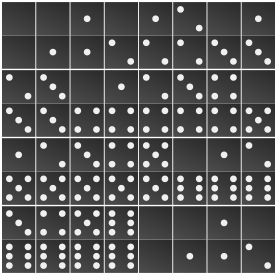
\includegraphics[scale=.9]{Bilder/Dominosteine.pdf}

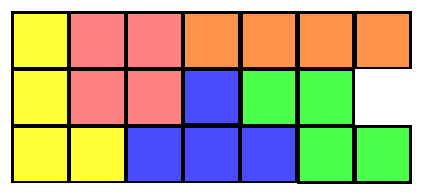
\includegraphics[scale=.9]{Bilder/Tetrominos-kompakt.pdf}

\includegraphics[scale=.9]{Bilder/ViererSchachbrett1.pdf}
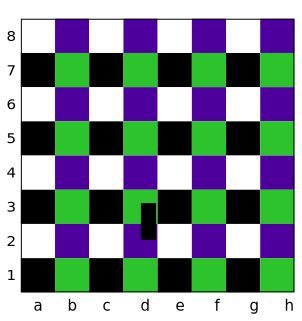
\includegraphics[scale=.9]{Bilder/ViererSchachbrett2.pdf}


\end{document}